% Тип документа
\documentclass[a4paper,12pt]{extarticle}

% Шрифты, кодировки, символьные таблицы, переносы
% \usepackage{cmap}
% \usepackage[T2A]{fontenc}
\usepackage[utf8]{inputenc}
\usepackage[russian]{babel}
% Это пакет -- хитрый пакет, он нужен но не нужен
\usepackage[mode=buildnew]{standalone}

\usepackage
	{
		% Дополнения Американского математического общества (AMS)
		amssymb,
		amsfonts,
		amsmath,
		amsthm,
		% Пакет для физических текстов
		physics,
		% misccorr,
		% 
		% Графики и рисунки
		wrapfig,
		graphicx,
		subcaption,
		float,
		tikz,
		tikz-3dplot,
		caption,
		csvsimple,
		color,
		booktabs,
		geometry,
		% 
		% Таблицы, списки
		makecell,
		multirow,
		indentfirst,
		%
		% Интегралы и прочие обозначения
		ulem,
		esint,
		esdiff,
		% 
		% Колонтитулы
		fancyhdr,
	} 
    
\usepackage{mathtools}
\mathtoolsset{showonlyrefs=true} 
\usepackage{pgfplots,pgfplotstable,booktabs,colortbl}
\usepackage{xcolor}
\usepackage{hyperref}
\usepackage{pythontex}
 % Цвета для гиперссылок
\definecolor{linkcolor}{HTML}{000000} % цвет ссылок
\definecolor{urlcolor}{HTML}{799B03} % цвет гиперссылок
 
\hypersetup{pdfstartview=FitH,linkcolor=linkcolor,urlcolor=urlcolor, colorlinks=true}
\hypersetup{pageanchor=false}
% Увеличенный межстрочный интервал, французские пробелы
\linespread{1.3} 
\frenchspacing 

\newcommand{\mean}[1]{\langle#1\rangle}

\begin{pycode}
##
def frexp10(decimal):
	parts = ('%e' % decimal).split('e')
	return float(parts[0]), int(parts[1])
##
\end{pycode}



% Функция для тех, кто использует pythontex. Представляет любое вещественное число в стандартном виде.
\newcommand{\frexp}[1]{
		\pyc{#10=frexp10(#1)} 
			\py{ round(#10[0],2)} 
				\cdot 10^{\py{#10[1]}} }

% const прямым шрифтом
\newcommand\ct[1]{\text{\rmfamily\upshape #1}}
\newcommand*{\const}{\ct{const}}
\usepackage{array}
\usepackage{pstool}

\geometry		
	{
		left			=	2cm,
		right 			=	2cm,
		top 			=	2.5cm,
		bottom 			=	2.5cm,
		bindingoffset	=	0cm
	}

%%%%%%%%%%%%%%%%%%%%%%%%%%%%%%%%%%%%%%%%%%%%%%%%%%%%%%%%%%%%%%%%%%%%%%%%%%%%%%%
	%применим колонтитул к стилю страницы
\pagestyle{fancy} 
	%очистим "шапку" страницы
% \fancyhead{} 
	%слева сверху на четных и справа на нечетных
\fancyhead[R]{}%\labauthors 
	%справа сверху на четных и слева на нечетных
% \fancyhead[L]{Отчёт по лабораторной работе №\labnumber}
\fancyhead[L]{\labtheme} 
	%очистим "подвал" страницы
% \fancyfoot{} 
	% номер страницы в нижнем колинтуле в центре
\fancyfoot[C]{\thepage} 

%%%%%%%%%%%%%%%%%%%%%%%%%%%%%%%%%%%%%%%%%%%%%%%%%%%%%%%%%%%%%%%%%%%%%%%%%%%%%%%

\renewcommand{\contentsname}{Оглавление}
\usepackage{tocloft}
\usepackage{secdot}
\sectiondot{subsection}


\begin{document}
\def\labauthors{Виноградов И.Д., Карусевич А.А., Понур К.А., Шиков А.П.}
\def\labgroup{440}
\def\labnumber{1}
\def\labtheme{Оценивание параметров случайного процесса}
\def\department{Кафедра статистической радиофизики}
\newcommand{\D}[1]{D\qty[#1]}
\begin{titlepage}

\begin{center}

{\small\textsc{Нижегородский государственный университет имени Н.\,И. Лобачевского}}
\vskip 1pt \hrule \vskip 3pt
{\small\textsc{Радиофизический факультет}}



\vfill
{\Large {\department}}

{\Large Отчет по лабораторной работе №\labnumber\vskip 12pt\bfseries \labtheme}
	
\end{center}

\vfill
	
\begin{flushright}
	{Выполнили студенты \labgroup\ группы \\ \labauthors}
\end{flushright}
	
\vfill
	
\begin{center}
	Нижний Новгород, \the\year
\end{center}

\end{titlepage}


\newpage
В настоящей работе изучаются вопросы, связанные с оценкой параметров случайных процессов, на примере оценки его среднего значения (математического ожидания). Это вполне оправданно, поскольку, во-первых, все принципиальные вопросы, возникающие при оценке параметров случайных процессов, проявляются уже в этой задаче. Во-вторых, при желании оценить другие параметры процесса чаще всего поступают следующим образом – подвергают случайный процесс такому преобразованию, при котором информация об интересующем параметре исходного процесса переходит в значение математического ожидания процесса преобразованного, и таким образом вопрос оказывается сведенным к оценке среднего значения преобразованного процесса.
Вопросы, связанные с оценкой параметров эргодических случайных процессов достаточно подробно рассмотрены в учебном пособии, с которым необходимо познакомиться перед выполнением настоящей работы.

При оценке того или иного параметра случайного процесса следует:
\begin{enumerate}
    \item Выбрать алгоритм оценки параметра (записать формулу, которая показывает, какие действия нужно производить с числами $x_{1},x_{2},\dots,x_n$ -- результатами измерений), чтобы получить число, принимаемое нами за оценку интересующего нас параметра.
    \item Исследовать выбранный алгоритм на предмет качества оценок. Качество оценки характеризуют ее \textbf{несмещенность}, \textbf{состоятельность} и \textbf{эффективность}:
    \begin{enumerate}
        \item Оценка называется \textbf{несмещенной}, если среднее статистическое её равно оцениваемой величине:  $\mean{\tilde a} = a$, где $a$ -- измеряемый параметр случайного процесса,  - его оценка\footnote{Оценка неизвестного параметра $a$ одним числом называется точечной}. Несмещенность оценки эквивалентна отсутствию систематической ошибки при измерении как в сторону ее завышения, так и в сторону ее занижения.
    \item Оценка называется состоятельной, если при неограниченном росте объёма экспериментального материала дисперсия оценки стремится к нулю. При этом вероятность сколь угодно малых отклонений оценки от оцениваемой величины тоже стремится к нулю. Таким образом, если оценка состоятельна, то можно быть уверенным, что величина ошибки измерения не превосходит допустимую при достаточно большом, но ограниченном объеме статистического материала (т.е. достаточно большом времени измерения).
    \item Если при измерении одной и той же характеристики случайного процесса можно пользоваться различными оценками, то эффективной называют оценку с наименьшей дисперсией. На практике не всегда удаётся удовлетворить всем этим требованиям. Например, может оказаться, что эффективная оценка существует, но формулы для её вычисления слишком сложны. Тогда приходится довольствоваться другой оценкой с несколько большей дисперсией. Иногда, в целях упрощения расчетов, применяются смещенные оценки. Но всегда выбору оценки должно предшествовать критическое изучение ее свойств.
    \end{enumerate}
\item Определить погрешность оценки параметра. 
\end{enumerate}
\section{Алгоритм оценки среднего значения}%
\label{sec:algoritm_otsenki_srednego_znacheniia}
Пусть мы имеем дело со случайной величиной $X$ и хотим найти её математическое ожидание.
Алгоритм оценки среднего значения выбирается в виде:
\begin{equation}
    \label{eq:1.1}
    \tilde x = \frac{1}{n} \sum\limits_{i=1}^{n} x_i \text{ для случайной величины)},
\end{equation}
где $x_i,~x_k$ -- результаты независимых измерений случайной величины;
\begin{equation}
    \label{eq:1.2}
    \tilde x = \frac{1}{n} \sum\limits_{i=1}^{n} x_i(t_i) \text{ (для случайного процесса)},
\end{equation}
где $x_i(t_i)$ -- дискретные выборки значений процесса $x(t)$, взятые в дискретные,
равноотстоящие на величину $\Delta t$, моменты времени ($\Delta t = t_{i+1}-t_i$ ).
Этот алгоритм оценки естественен, поскольку известно, что $\frac{1}{n} \sum\limits_{i=1}^{n} x_i$-- среднеарифметическое $n$ независимых измерений случайной
величины -- сходится по вероятности к среднему значению $\mean{x}^2$ (математическому
ожиданию) при $n \to \infty $.

Нетрудно показать, что оценки среднего \eqref{eq:1.1}, \eqref{eq:1.2}  являются
\textbf{несмещенными} (т.е. не содержат систематической ошибки). Действительно, проводя
статистическое усреднение левых и правых частей и учитывая эргодичность изучаемого
случайного процесса, получаем $\mean{\tilde x} = \mean{x}$, т.е. статистическое среднее оценок равно среднему
статистическому самого процесса.

При получении оценки среднего значения стационарного эргодического процесса согласно 
\eqref{eq:1.2}, усредняются дискретные выборочные значения процесса, отстоящие во времени 
на $\Delta t$. Возникает закономерный вопрос, не проигрываем ли мы в чем то существенном,
не используя информацию о процессе, заключающуюся в промежуточных значениях процесса,
лежащих между дискретными отсчетами. Может быть, оценка среднего существенно улучшится,
если взять ее в виде непрерывного усреднения реализации процесса на некотором временном 
интервале, длительностью $T$, примыкающем к текущему моменту времени $t$:
\begin{equation}
    \label{eq:1.3}
    \tilde x(t) = \frac{1}{T} \int\limits_{t-T}^{t} x(\tilde t) \dd{\tilde t} 
\end{equation}

В связи с тем, что при использовании численных методов сам интеграл в \eqref{eq:1.3}
вычисляется приближенно через значения подынтегральной функции в отдельных дискретных точках. Оценку 
\eqref{eq:1.3}  можно рассматривать как частный случай оценки \eqref{eq:1.2},
если отсчеты берутся достаточно часто (если интервал между отсчетами существенно меньше 
времени корреляции процесса $\Delta t \ll \tau_{\text{кор}}$). Тем не менее, имеет смысл
рассмотреть аналитически [1] оценку среднего в виде (1.3) и убедиться в том, что величина
погрешности оценки определяется лишь числом некоррелированных отсчетов содержащихся в 
интервале усреднения $T$.
Другими словами, если в оценке \eqref{eq:1.1}  взято $n$ некоррелированных отсчетов, а в
оценке \eqref{eq:1.3}  интервал усреднения $T$ выбран равным $T = n \tau_{\text{кор}}$,
оценки \eqref{eq:1.1}  и \eqref{eq:1.3}  оказываются эквивалентными по точности при $n\gg 1$. Следует проследить за выполнением этого утверждения при выполнении заданий №3,5.

\section{Погрешность оценки}%
\label{sec:pogreshnost_otsenki}
На практике важно не просто получить оценку параметра, но и оценить, как близко значение оценки к истинному значению параметра. Другими словами, необходимо оценить погрешность оценки. Поскольку конкретное значение оценки параметра случайно (оно определяется конкретной выборкой $x_{1},x_{2},\dots,x_n$), то и ошибка конкретной оценки тоже случайна. Поэтому при рассмотрении погрешности оценки имеется в виду рассмотреть ее поведение на ансамбле независимых замеров оценки.

За погрешность оценки принимаем среднеквадратическое отклонение оценки от среднего
значения (корень квадратный из дисперсии оценки), т.е.
\begin{equation}
    \label{eq:2.1}
    \sigma_{\tilde x} = \sqrt{ D\qty[\tilde x]} = \sqrt{ \mean{(\tilde x - \mean{x})^2} }
\end{equation}
или средний квадрат отклонения от истинного среднего. С.К.О. оценки показывают в каком интервале
лежат оценки среднего.

В предельном случае при $n=1$, (производится \textbf{однократный отсчёт}), и результат $x_{1}$ принимается за оценку среднего), ошибка конкретной оценки  $(x_{1}-\mean{x})$ естественно будет случайной,
а погрешность оценки:
\begin{equation}
    \label{eq:2.2}
    \sqrt{ \mean{ \qty( x_{1} - \mean{x} )^2 } } = \sqrt{D\qty[x]} = \sigma_x
\end{equation}

Из \eqref{eq:2.2} видно, что мерой погрешности оценки при $n=1$ является 
среднеквадратическое отклонение (СКО) исследуемой случайной величины (корень квадратный из дисперсии
исходного процесса в случае \eqref{eq:1.1} ).

Известно, что при усреднении <<$n$>> независимых одинаково распределенных
слагаемых дисперсия уменьшается в $n$ раз
\begin{equation}
    \label{eq:2.3}
    \sigma_{\tilde x} = \sqrt{ \frac{D\qty[x] }{n}}
\end{equation}

Если же оценивается среднее значение эргодического процесса, согласно алгоритму
\eqref{eq:1.2}, дисперсию оценки $D\qty[\tilde x] = \mean{ \qty( \tilde x - \mean{x} )^2 }$
можно записать [1] в виде
\begin{equation}
    \label{eq:2.4}
    D\qty[\tilde x] = \frac{\D{x}}{n} + \frac{1}{n^2} \sum\limits_{i=1}^{n} \sum\limits_{j\neq i}^{n} B_x(t_i - t_j),
\end{equation}
где $B_x(t_i - t_j) = \mean{ (x_i - \mean{x}) (x_i - \mean{x})  }$ -- функция
ковариации процесса  $x(t)$, причем $\D{x}$ -- дисперсия процесса $x(t)$ -
равна $\D{x}=B_x(0)$.

При $n \to \infty$ дисперсия оценки стремится к нулю $\D{\tilde x} \to 0$, т.е.
оценка является \textbf{состоятельной}.

Из \eqref{eq:2.4} видно, что величина $\D{\tilde x}$ дисперсии оценки \eqref{eq:1.2} 
существенно зависит от степени коррелированности отсчетов, а значит от того, насколько
велик интервал между отсчетами $\Delta t$ по сравнению с $\tau_{\text{кор}}$ - временем
корреляции процесса ( $t_{\text{кор}}$ -- эффективная протяженность $B_x(\tau)$ - 
функции ковариации процесса $x(t)$ ).


Здесь есть две предельные ситуации:
\begin{enumerate}
    \item Все $n$ отсчетов укладываются на времени, существенно меньшем времени корреляции
        процесса ($n\cdot \Delta t \ll \tau_{\text{кор}}$), тогда дисперсия оценки равна
        дисперсии исходного процесса $\D{\tilde x}= \D{x}$. В этом случае <<n>> отсчетов
        по влиянию на точность оценки эквивалентны одному отсчету.
    \item  Если же $\Delta t \geq \tau_{\text{кор}}$, то можно принять  и дисперсия оценки \eqref{eq:1.2} 
        оказывается равной, т.е. дисперсия оценки аналогично \eqref{eq:2.3}  в <<n>> раз уменьшается по сравнению с дисперсией процесса, где <<n>> ‑ число некоррелированных отсчетов в оценке \eqref{eq:1.2} .

Поведение СКО оценки при произвольных $\Delta t$ исследуется в заданиях №№ 3, 4.
\end{enumerate}


\section{Оценка среднего значения и погрешности оценки среднего при помощи спектральной 
плотности мощности}%

Как уже рассматривалось выше, если $x(t)$ -- случайный эргодический процесс, то среднее
$\mean{x}$ может быть найдено путем усреднения по времени в виде \eqref{eq:1.3}.

Корреляционная функция процесса $x(t)$ :
\begin{equation}
    \label{eq:}
    K_x\qty[\tau] = B_x[\tau] + \mean{x}^2,
\end{equation}
а спектральная плотность мощности:
\begin{equation}
    \label{eq:}
    S_x(\omega) = S_{x-\mean{x}}(\omega) + 2 \pi \delta(\omega) \mean{x}^2.
\end{equation}
Т.е. в случае ненулевого среднего значения в спектре случайного процесса наблюдается $\delta$ - 
функция на нулевой частоте, а дисперсия представляет собой площадь под непрерывной частью спектра.

Оценку среднего значения процесса в виде \eqref{eq:1.3}  можно рассматривать, как некоторый новый процесс,
полученный из исходного путем линейного преобразования. В задании №5 рассматривается спектральная плотность мощности  оценки  в виде \eqref{eq:1.3} . Как найти по  погрешность оценки \eqref{eq:1.3}. Исследовать, как изменяется  с увеличением времени усреднения $T$, за счет чего при этом уменьшается погрешность оценки среднего.
Для объяснения результатов этого задания, необходимо иметь в виду, что спектральная плотность мощности оценки среднего значения в виде \eqref{eq:1.3} , т.е. $S_{\tilde x}(\omega)$, связана со спектральной плотностью мощности исходного процесса $S_x(\omega)$  соотношением
\begin{equation}
    \label{eq:4.1}
    S_{\tilde x}(2 \pi f) = S_x(2 \pi f) \abs{K(j 2 \pi f)}^2
\end{equation}

Коэффициент передачи  $K(j 2 \pi f)$ линейного преобразования \eqref{eq:1.3}  можно найти, как комплексную амплитуду выходного гармонического колебания, если же вместо входного 
процесса  $\tilde x(t)$ в \eqref{eq:1.3}  подставить $e^{j 2 \pi f t}$ (гармоническое колебание единичной амплитуды и частоты $2 \pi f$). При этом окажется, что 
\begin{equation}
    \label{eq:4.2}
    \abs{K(j_{2} \pi f)}^2 = \abs{\frac{\sin{\pi f T}}{\pi f T}}^2
\end{equation}

Из \eqref{eq:4.2}  видно, что усреднитель \eqref{eq:1.3} действует как фильтр,
пропускающий спектральные составляющие в эффективной полосе $\Delta f_x = \frac{1}{2T}$,
примыкающей к $f=0$. Постоянная составляющая, а также $S_{\tilde x}(0)$ спектральная плотность
мозности процесса $\tilde x(t)$ на нулевой частоте, при этом остаются неизменными, т.к.
$K(j 2 \pi f) \eval_{f=0}=1$. С увеличением $T$, уменьшается полоса пропускания этого фильтра,
а значит и $\D{\tilde x}$ -- дисперсии оценки \eqref{eq:1.3},
приближенно равная $\D{\tilde x}=S_{\tilde x}(0)\cdot \Delta f_{\tilde x} = S_{\tilde x}(0) \frac{1}{2T}$.

При выполнении задания №5 следует убедиться, что $\D{\tilde x} = \frac{\D{x}}{T / \tau_{\text{кор}}}$, (при $T\gg \tau_{\text{кор}}$ ), т.е.
погрешность оценки \eqref{eq:1.3} определяется только числом некоррелированных отсчетов,
содержащихся в интервале усреднения $T$.

В этом задании следует получить так же оценку среднего значения и оценить ее 
погрешность непосредственно по спектральной плотности мощности процесса $\tilde x(t)$. 
Эта оценка оказывается по существу эквивалентной оценке \eqref{eq:1.3}  при времени усреднения $T$,
равном тому временному интервалу $T^*$, на котором мы находим Фурье-преобразование процесса 
(в нашем случае $T^*=2048$); а ширина спектральной плотности мощности оценки, определяющая 
ее дисперсию, обратна длине этого интервала и равна $1/2048$ (по существу это ширина 
интервала частотного разрешения в спектре при выбранных параметрах Фурье-преобразования).

\section{Доверительный интервал и доверительная вероятность}%
\label{sec:doveritel_nyi_interval_i_doveritel_naia_veroiatnost_}
Выше за количественную характеристику погрешности оценки среднего значения было взято СКО 
оценки (корень квадратный из дисперсии оценки). Но в связи с тем, что оценка является 
случайной величиной, определяемой случайными выборочными значениями $x_1,x_2,\dots,x_n$,
на практике возможна реализация таких значений оценки, которые отличаются от истинного
значения среднего больше, чем на величину СКО оценки. Как часто это может происходить, и
какой должна быть выбрана длина интервала, характеризующего погрешность оценки, чтобы с
достоверностью неизвестное среднее отстояло от случайной оценки не дальше, чем на величину 
выбранного интервала? Сначала несколько слов о том, что значит с достоверностью? При какой 
вероятности появление события его можно считать практически достоверным? Эта вероятность 
определяется существом исходной задачи. В некоторых задачах это может быть $0.90$ или $0.95$; $0.99$ и т.д. Эту вероятность будем называть доверительной и обозначать $\beta$. 
По этой вероятности выбирается $I_{\beta}$ величина интервала, называемого доверительным 
(обычно его длина выражается в долях среднеквадратического значения оценки $I_{\beta}=t_{\beta} \sigma_{{\tilde x}}$). 
Если отложить этот интервал вокруг случайного значения оценки, то он с доверительной 
вероятностью $\beta$ накроет неизвестное среднее значение $\mean{x}$ (т.е. практически с достоверностью).

Величина доверительного интервала выражается через плотность вероятностного распределения о
оценки $W(\tilde x)$ и доверительную вероятность $\beta$ согласно соотношению:
\begin{equation}
    \label{eq:5.1}
    P\qty(\abs{\mean{x}} - \tilde x \leq I_{\beta}) = \int\limits_{\mean{x}-I_{\beta}}^{\mean{x}+I_{\beta}}  W(\tilde x) \dd{\tilde x} = \beta
\end{equation}

В значительном ряде случаев принимается, что плотность вероятности оценки  $W(\tilde x)$ распределена по закону Гаусса (по закону Гаусса зачастую распределена и сама величина $X$,
среднее значение которой оценивается, но если $X$ не имеет гауссова распределения, то 
можно принять распределенной по закону Гаусса саму оценку $\tilde x$  при достаточно большом числе 
усредняемых некоррелированных слагаемых в \eqref{eq:1.1}  в силу центральной предельной теоремы теории вероятностей).
При небольших $n$ ($n\leq 15$ ) распределение оценки $\tilde x$ нельзя считать 
Гауссовым даже в том случае, когда $X$ -- распределено по закону Гаусса, если 
неизвестна дисперсия величины $X$ и она оценивается по тем же <<n>> отсчетам. 
Подробнее об этом сказано в примечании к заданию №6. 
В этом случае следует находить доверительный интервал для оценки, считая, что относительная величина оценки $\frac{\tilde x}{\sigma_{\tilde x}}$ распределена по
закону Стьюдента с числом степеней свободы равным <<n-1>> (где $n$ -- число 
усредняемых некоррелированных отсчетов в оценке \eqref{eq:1.1}  и, пользуясь соответствующими таблицами, имеющимися в справочной литературе).

Вопросы, связанные с описание погрешности оценки через доверительный интервал и доверительную вероятность, рассматриваются в задани  №6.

\section{Практическая часть}
\subsection[Задание 1]{Вид реализации случайных процессов и их спектров}

Порядок действий:
\begin{enumerate}
	\item Установили в Генераторе сигналов соответствующее время корреляции Гауссова шума $\tau_\text{кор} = 10$
	\item В блоке Анализатор выбрали график реализации сигнала “Реализация”, или спектр сигнала “СПМ”
	\item Нажали кнопку “Run”
\end{enumerate}
Пронаблюдали вид реализаций и спектральную плотность мощности изучаемого Гауссова шума с различным временем корреляции $\tau_\text{кор} =10; 30; 100$.

 Ниже приведены полученные графики реализации процесса
 \begin{figure}[H]
 	\begin{minipage}{0.3\linewidth}
 		\centering
        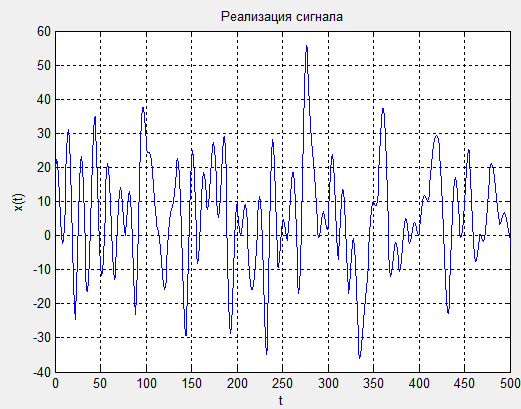
\includegraphics[width=\linewidth]{fig/fig1_t10}
 		\caption*{$\tau_\text{кор}=10$}
 	\end{minipage}
 \begin{minipage}{0.3\linewidth}
 	\centering
    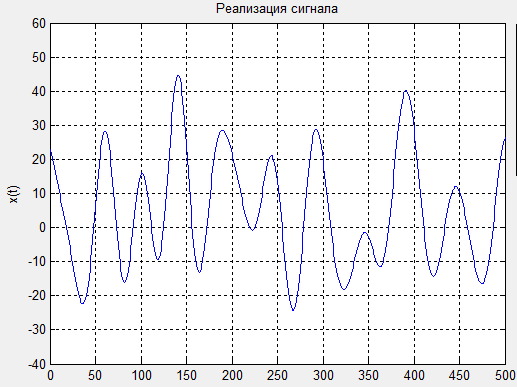
\includegraphics[width=\linewidth]{fig/fig1_t30}
 	\caption*{$\tau_\text{кор}=30$}
 \end{minipage}
\begin{minipage}{0.3\linewidth}
	\centering
    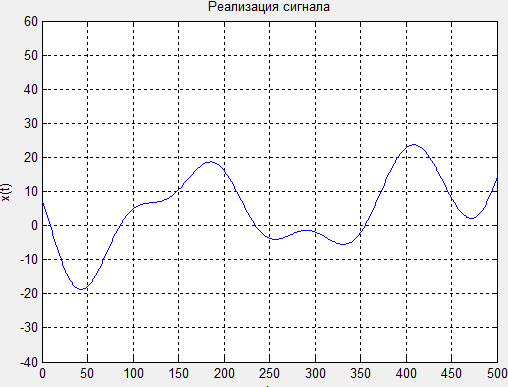
\includegraphics[width=\linewidth]{fig/fig1_t100}
	\caption*{$\tau_\text{кор}=100$}
\end{minipage}
  \end{figure}
и его спектральной плотности мощности
 \begin{figure}[H]
	\begin{minipage}{0.3\linewidth}
		\centering
        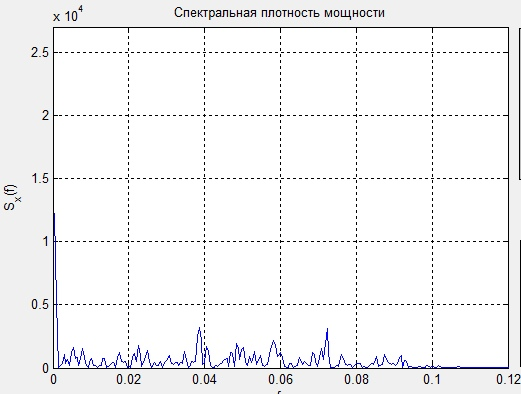
\includegraphics[width=\linewidth]{fig/realize10_sp.jpg}
		\caption*{$\tau_\text{кор}=10$}
	\end{minipage}
	\begin{minipage}{0.3\linewidth}
		\centering
        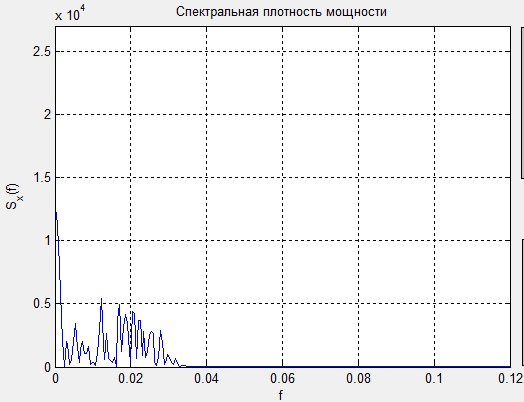
\includegraphics[width=\linewidth]{fig/realize30_sp.jpg}
		\caption*{$\tau_\text{кор}=30$}
	\end{minipage}
	\begin{minipage}{0.3\linewidth}
		\centering
        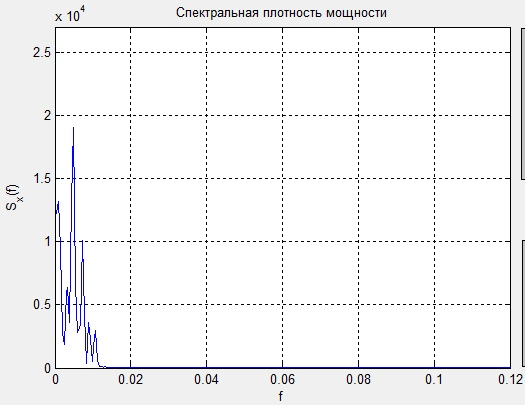
\includegraphics[width=\linewidth]{fig/realize100_sp.jpg}
		\caption*{$\tau_\text{кор}=100$}
	\end{minipage}
\end{figure}
\paragraph{Вывод} Установили, что с увеличением времени корреляции $\tau_\text{кор}$ в спектре становится меньше гармоник, он сужается.

Так как $\tau_\text{кор}$ - интервал времени, на котором ф-я корреляции $B(\tau)$ уменьшается в $e$ раз, то время
корреляции определяет, насколько в случайном процессе каждое следующее во времени его значение связано с предыдущим. 
При небольшом времени корреляции - каждое следующее значение случайного процесса слабо зависит от предыдущего, что и
продемонстрировано в эксперименте при $\tau_\text{кор}=10$, где наблюдается высокоосциллирующая реализация.

При увеличении $\tau_\text{кор}$, значения процесса больше зависят от предыдущих, поэтому при
$\tau_\text{кор} = 100$ мы наблюдаем более плавную реализацию. Реализации процесса с увеличением времени корреляции
слабее меняются во времени.


\subsection[Задание 2]{Поведение оценки среднего в зависимости от числа усредняемых отсчетов}
Порядок действий:
Сначала определили оценки среднего и среднеквадратического отклонения оценки процесса по ансамблю
\begin{enumerate}
	\item Установили в Генераторе сигналов соответствующее время корреляции Гауссова шума $\tau_\text{кор} = 10$
	\item В Усреднителе выбрали количество реализаций М = 256, время между отсчетами $\Delta t = 1$, и количество усредняемых отсчетов N = 1.
	\item 	В Блоке оценок определили оценку среднего и С.К.О. оценки.	
	\begin{figure}[H]
		\centering
        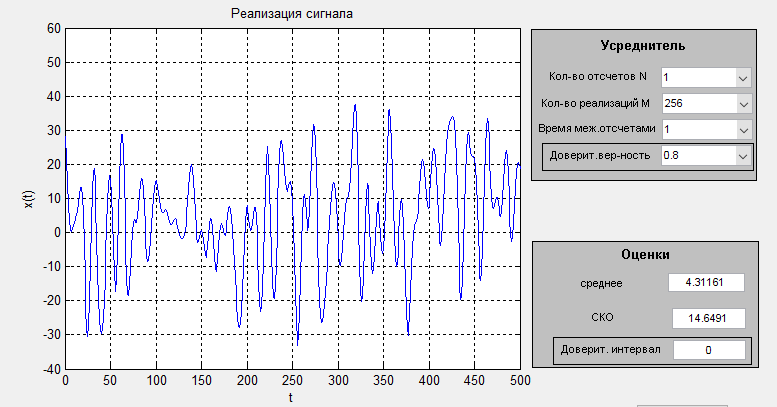
\includegraphics[width=\linewidth]{fig/fig21}
	\end{figure}

	Далее определили оценки по реализациям:
	\item Установили в Генераторе сигналов соответствующее время корреляции Гауссова шума $\tau_\text{кор} = 10$
	\item В Усреднителе выбрали количество реализаций М = 8, время между отсчетами $\Delta t = 1$, и количество усредняемых отсчетов N = 128.
	\item Нажали на кнопку “Усреднение”, и в блоке Анализатор выбрали график “Среднее” (на графике $N$ - текущее количество отсчетов по которым производится усреднение).
	\begin{figure}[H]
		\centering
        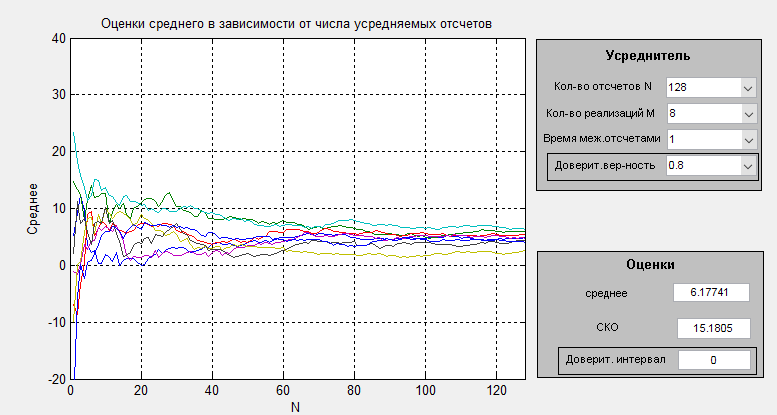
\includegraphics[width=\linewidth]{fig/fig22}
	\end{figure}

Разброс оценки $\mean{x}$ по вертикали при фиксированном $N$ характеризует собой погрешность оценки среднего при данном $N$. 
Оценим этот разброс при $N=1, N=40, N=128$, приблизив график (в программе) и найдя крайние значения. ??

\begin{table}[h!]
	\centering
	\begin{tabular}{|c|c|c|}
		\hline
		\textbf{Количество отсчетов} & \textbf{Крайние значения} &{\textbf{Разброс $\mean{x}$ по вертикали}} \\
		\hline
		N=1   & От -25 до 25 & 50 \\
		\hline
		N=40  & От 2 до 9 & 7 \\
		\hline
		N=128 & От 2.5 до 6.25 & 3.75 \\
		\hline
	\end{tabular}%
\end{table}%
\end{enumerate}




\subsection[Задание 3]{Изучение зависимости $\sigma$ -- среднеквадратичного отклонения оценки среднего от числа усреднений в оценке}
Порядок действий:
\begin{enumerate}
	\item Для корректного отображения графиков перед экспериментом очистили область построения графиков кнопкой «Reset».
	\item Установили в Генераторе сигналов соответствующее время корреляции Гауссова шума.
	\item В Усреднителе выбрали количество реализаций М = 256 (это необходимо для того, чтобы кривые зависимостей получались гладкими), количество усредняемых отсчетов N = 64, а время между отсчетами первоначально взяли $\Delta t = 1$.
	\item Нажали на кнопку «Вычисление С.К.О.» («СКО(N)»).
	\item Для получения следующего графика в серии, в Усреднителе изменили время между отсчетами усреднения $\Delta t$ в
	соответствии с заданием и нажали на кнопку «Вычисление С.К.О.» («СКО(N)»).
	\item Для перехода к следующей серии нажали «Сброс» (Reset), а в Генераторе сигналов изменили время корреляции и повторили пункты 3) и 4).
\end{enumerate}
В результате эксперимента получили две серии графиков по три графика в серии, отличающиеся временем между отсчетами $\Delta t=1; 4; 12$.
Для первой серии время корреляции $\tau_\text{кор} = 10$. Для второй серии время корреляции $\tau_\text{кор} = 100$.
Ниже представлены эти серии.
\begin{figure}[H]
    \begin{minipage}{0.49\linewidth}
        \centering
        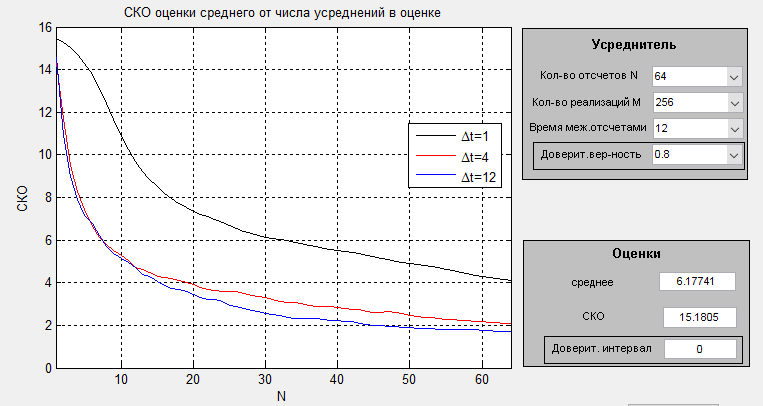
\includegraphics[width=0.95\linewidth]{fig/fig31}
        \caption*{$\tau_\text{кор} = 10$}
    \end{minipage}
    \begin{minipage}{.49\linewidth}
        \centering
        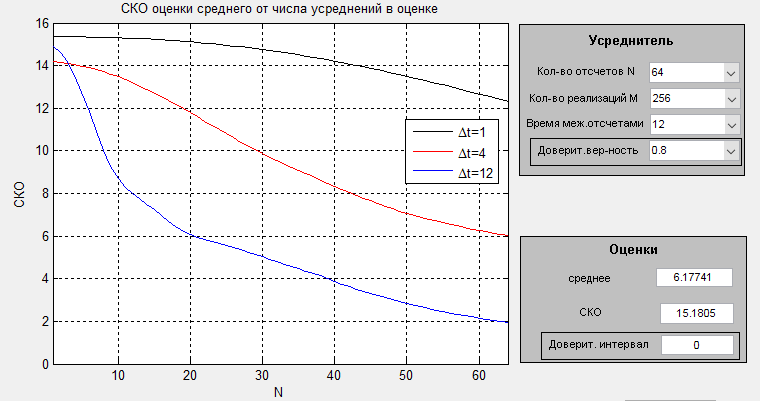
\includegraphics[width=0.95\linewidth]{fig/fig32}
        \caption*{$\tau_\text{кор} = 100$}
    \end{minipage}
	\caption{}
	\label{fig:3}
\end{figure}
Разберем качественно поведение кривых на рис.\ref{fig:3} 
\begin{enumerate}
	\item Нулевая производная при $N=1$ объясняется тем, что при любом количестве отсчетов $N>1$, при том же
	количестве реализаций $M$, значение оценки среднего будет ближе к истинному значению мат. ожидания, а СКО оценки - уменьшаться. Таким
	образом, при $N=1$ наблюдается максимум СКО оценки среднего.
    \item Можно показать, что с ростом времени корреляции СКО оценки среднего должны уменьшаться, поскольку оценка среднего совпадет с истинным значением при
        \begin{equation}
            \label{eq:}
            \tilde x(t) = \lim_{T \to \infty} \int\limits_{0}^{T = n\cdot \tau_{\text{кор}}}  x(t) \dd{t}
		\end{equation}
		то увеличивая время корреляции мы сильнее приближаемся к условию $T \to \infty$, а значит СКО оценки должен уменьшаться.
	\item Оценим время корреляции процесса непосредственно по графику. Так как в случае $\Delta t \ge \tau_\text{кор}$ СКО
	оценки можно рассчитывать как $D[\tilde{x}] = \frac{D[x]}{N}$, то график СКО оценки от числа отсчетов после
	прохождения точки $\Delta t * N = \tau_\text{кор}$ будет вести себя как гипербола. По точке перехода графика в гиперболу
	можно определить $\tau_\text{кор}$.
	\item СКО оценки при $N=1$ определяется числом реализаций сигнала $M$. В таком случае для каждой
	реализации среднее значение - это значение единственного элемента в реализации. Другими словами, СКО оценки при
	$N=1$ определяется как дисперсия исходного процесса $D[x]$.
	
\subsection[Задание 4]{Изучение зависимости $\sigma$ -- среднеквадратичного отклонения оценки среднего от времени между отсчетами $\Delta t$}
Порядок действий
\begin{enumerate}
	\item Для корректного отображения графиков перед экспериментом очистили область построения графиков кнопкой «Reset».
	\item Установили в Генераторе сигналов соответствующее время корреляции Гауссова шума.
	\item В Усреднителе выбрали количество реализаций М = 256 (это необходимо для того, чтобы кривые зависимостей получались гладкими), а затем выбрали необходимое количество отсчетов усреднения ($N = 4; 32$).
	\item Нажали на кнопку “СКО($delta_{-}t$)”.
	\item Для получения следующего граф ка в серии, в Генераторе изменили время корреляции в соответствии с заданием и нажали на кнопку “СКО($delta_{-}t$)” («СКО(N)»)
	\item Для перехода к следующей серии ($N=32$) ) изменили в Усреднителе количество усреднений, нажали “Reset” в блоке Анализатор и повторить пункты 4) и 5).
\end{enumerate}
В результате эксперимента получили две серии графиков (с $N = 4$ и $N = 32$) по три графика в серии.
Получили серию кривых $\sigma(\Delta t)$, для процессов с различным временем корреляции $\tau_\text{кор}= 10; 30; 100$. Число усреднений в оценке среднего взяли равным $N = 4$ ($\Delta t$ на графиках изменяется в пределах от 1 до 32).
Вторую серию кривых получили для тех же времен корреляции $\tau_\text{кор}= 10; 30; 100$, а число усреднений в оценке среднего взяли $N = 32$.
Графики приведены ниже
\begin{figure}[H]
	\centering
    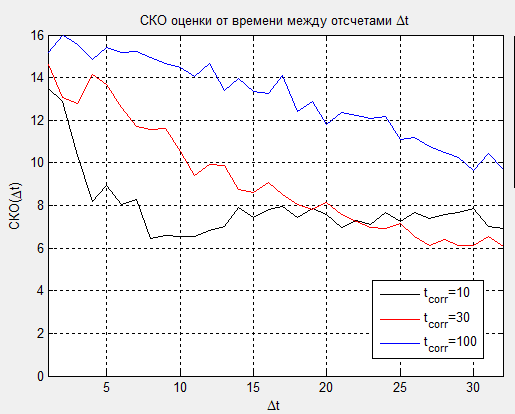
\includegraphics[width=.8\linewidth]{fig/fig41}
	\caption{$N = 4$}
    \label{fig:4.1}
\end{figure}

\begin{figure}[H]
	\centering
    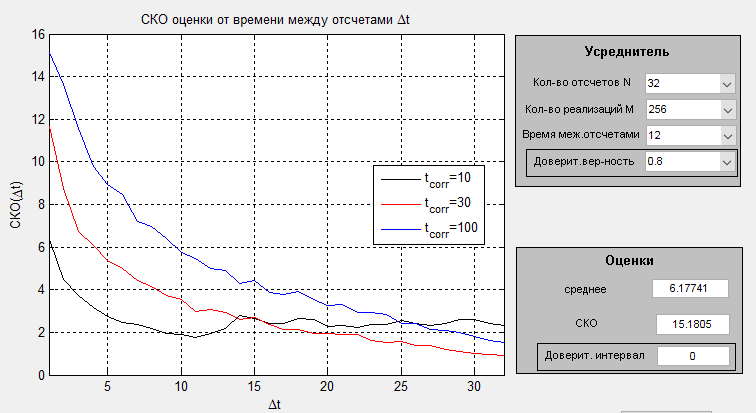
\includegraphics[width=\linewidth]{fig/fig42}
	\caption{$N = 32$}
    \label{fig:4.2}
\end{figure}
\end{enumerate}
\subsection[Задание 5]{Определение оценок среднего значения и среднеквадратического отклонения по спектральной плотности мощности (СПМ) процесса}
Оценку среднего значения процесса, найденную как среднее по времени на фиксированном по длине скользящем интервале усреднения, можно рассматривать как новый случайный процесс и для него можно найти спектральную плотность мощности.

Порядок действий
\begin{enumerate}
	\item Установили в Генераторе сигналов корреляции Гауссова шума $\tau_\text{кор}=10$.
\end{enumerate}
\subsubsection[Задание 5.1]{Определение параметров исходного процесса по его СПМ:}
\begin{enumerate}
	\item В блоке Анализатор выбрали график “Спектр сигнала” (“СПМ”) нажали кнопку «Run» и, согласно заданию, вычислили среднее сигнала, а затем дисперсию.
\end{enumerate}

\begin{figure}[H]
	\centering
    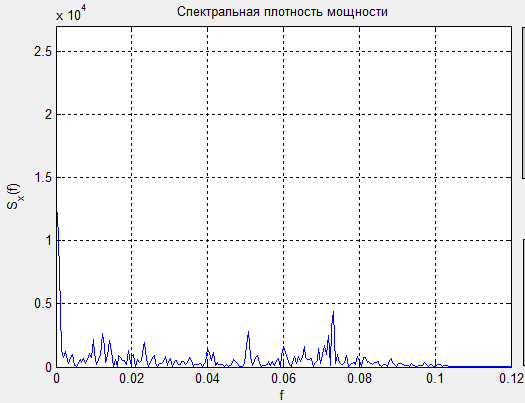
\includegraphics[width=0.8\linewidth]{fig/fig51}
	\caption*{$\tau_\text{кор} = 10$}
\end{figure}	


При изменении масштаба было найдено значение $S_x(0)=1,22\cdot 10^4$.

В связи с этим полная мощность в полосе  = 1/2048 на нулевой частоте равна (с некоторой погрешностью) $\mean{x}^2 = A\cdot \frac{1}{2048}$, где $А$ – значение СПМ на нулевой частоте по графику. Отсюда находим $\mean{x}$.

$\mean{x}^2 = S_x(0)\cdot \frac{1}{2048}= 1,22\cdot 10^4\cdot \frac{1}{2048} = 5,96$

$\mean{x} =  \sqrt{\mean{x}^2} = 2,44$

Дисперсию процесса по графику спектральной плотности мощности нашли как произведение эффективной ширины спектра на эффективное значение СПМ.

$D[\tilde{x}] = S_x(0)\cdot \Delta f_{\tilde{x}} =\frac{\mean{x}^2}{2} = 2,98$

$\sigma_{\tilde{x}} = \sqrt{D[\tilde{x}]}\approx 1,73$

Сравнили полученные результаты с данными из Задания 2.
\subsubsection[Задание 5.1]{Определение параметров усредненного процесса по его СПМ:}
\begin{enumerate}
	\item В Усреднителе установили количество реализаций М = 2 и время между отсчетами $\Delta t = 1$, а затем выбрали количество отсчетов усреднения N = 4.
	\item В блоке Анализатор выбрали график “Спектр усреднен.” (“Уср. СПМ”), нажали кнопку «Run», и, затем, аналогично заданию 5.1 вычислили оценку среднего значения и дисперсию оценки.
	\item Для проведения следующего эксперимента повторили пункты 3) и 4) для количества отсчетов усреднения N = 32.
\end{enumerate}
 \begin{figure}[H]
	\begin{minipage}{.45\linewidth}
		\centering
       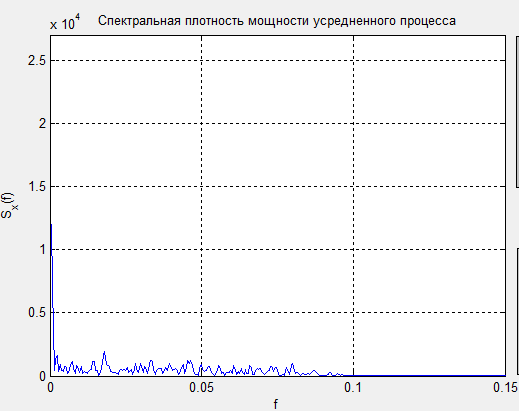
\includegraphics[width=\linewidth]{fig/fig52}
	\caption*{$N = 4$}
	\end{minipage}
	\begin{minipage}{.45\linewidth}
		\centering
        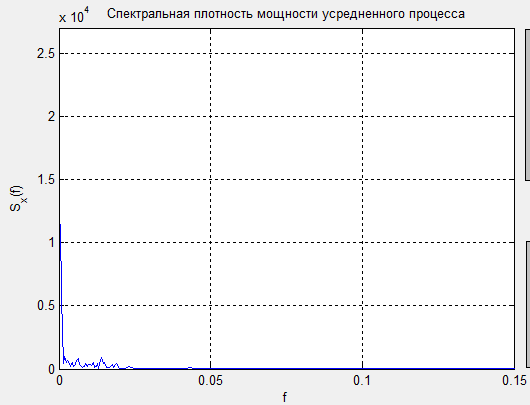
\includegraphics[width=\linewidth]{fig/fig53}
	\caption*{$N = 32$}
	\end{minipage}
\end{figure}
\paragraph{Для $N=4$}%


$S_x(0)=1,2\cdot 10^4$

$\mean{x}^2 = S_x(0)\cdot \frac{1}{2048}= 1,22\cdot 10^4\cdot \frac{1}{2048} = 5,86$

$\mean{x} =  \sqrt{\mean{x}^2} = 2,42$

$D[\tilde{x}] = S_x(0)\cdot \Delta f_{\tilde{x}} =\frac{\mean{x}^2}{2} = 2,93$

$\sigma_{\tilde{x}} = \sqrt{D[\tilde{x}]}\approx 1,71$

\paragraph{Для $N=32$}%
$S_x(0)=1,15\cdot 10^4$

$\mean{x}^2 = S_x(0)\cdot \frac{1}{2048}= 1,22\cdot 10^4\cdot \frac{1}{2048} = 5,62$

$\mean{x} =  \sqrt{\mean{x}^2} = 2,37$

$D[\tilde{x}] = S_x(0)\cdot \Delta f_{\tilde{x}} =\frac{\mean{x}^2}{2} = 2,8$

$\sigma_{\tilde{x}} = \sqrt{D[\tilde{x}]}\approx 1,68$

\subsection[Задание 6]{Описание погрешности и надежности оценки среднего значения через доверительный интервал и доверительную вероятность}
\subsubsection[Задание 6.1]{Анализ гистограммы}
Порядок действий:
\begin{enumerate}
	\item Установили в Генераторе сигналов время корреляции Гауссова шума $\tau_\text{кор}=10$.
	\item В Усреднителе выбрали количество реализаций М = 256 (это необходимо для того, чтобы кривые зависимостей получались гладкими), доверительную вероятность $\beta = 0.95$, время между отсчетами $\Delta t = 1$ и необходимое количество отсчетов усреднения $N=1$.
	\item Нажали кнопку “PDF”, и следили за изменением значения доверительного интервала в Блоке оценок.
	\item Для проведения следующего эксперимента повторили пункт 2), выбирая количество отсчетов усреднения, соответственно, N = 4; 32.
\end{enumerate}

 \begin{figure}[H]
	\begin{minipage}{.5\linewidth}
		\centering
       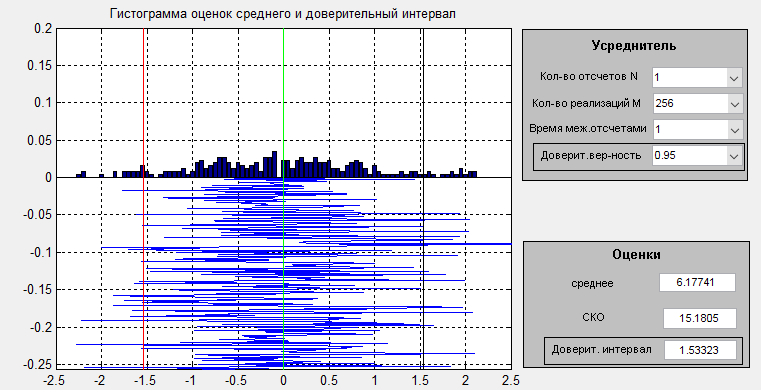
\includegraphics[width=\linewidth]{fig/fig61}
	\caption*{$N = 1$}
	\end{minipage}
	\begin{minipage}{.5\linewidth}
		\centering
        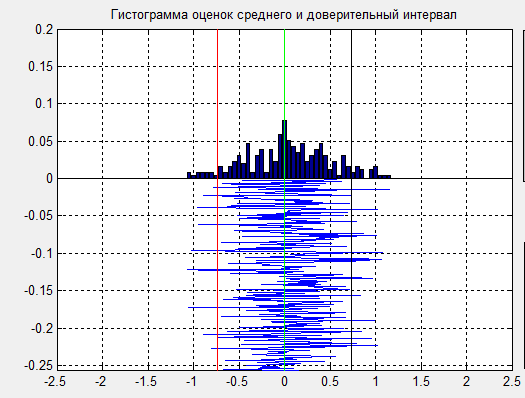
\includegraphics[width=\linewidth]{fig/fig62}
	\caption*{$N = 4$}
	\end{minipage}
	\begin{minipage}{.5\linewidth}
		\centering
        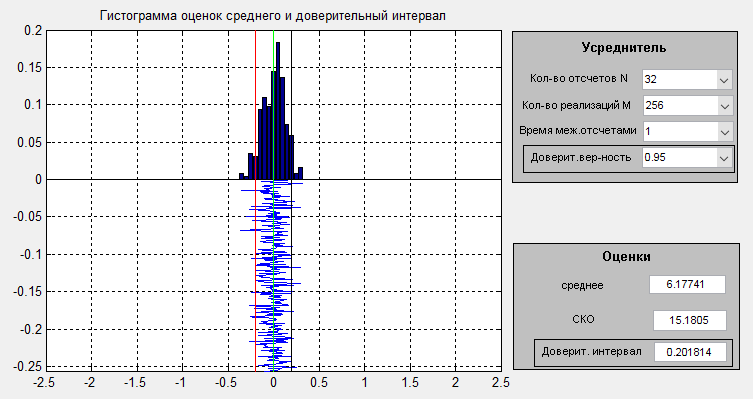
\includegraphics[width=\linewidth]{fig/fig63}
	\caption*{$N = 32$}
	\end{minipage}
	\begin{minipage}{.5\linewidth}
		\centering
        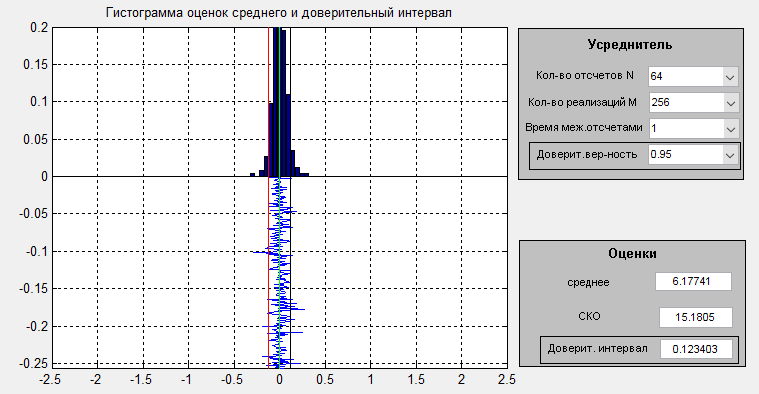
\includegraphics[width=\linewidth]{fig/fig64}
	\caption*{$N = 64$}
	\end{minipage}
\end{figure}
% Table generated by Excel2LaTeX from sheet 'task2'
\begin{table}[htbp]
	\centering
%	\caption{Add caption}
	\begin{tabular}{|c|c|}
		\toprule
		\multicolumn{1}{|c|}{\textbf{Количество отсчетов усреднения $N$}} & \textbf{Доверительный интервал $I$} \\
		\midrule
		1     & 1.5332 \\
		\midrule
		4     & 0.7248 \\
		\midrule
		32    & 0.2018 \\
		\midrule
		64    & 0.1234 \\
		\bottomrule
	\end{tabular}%
	\label{tab:addlabel}%
\end{table}%
 \begin{figure}[H]
	\centering
    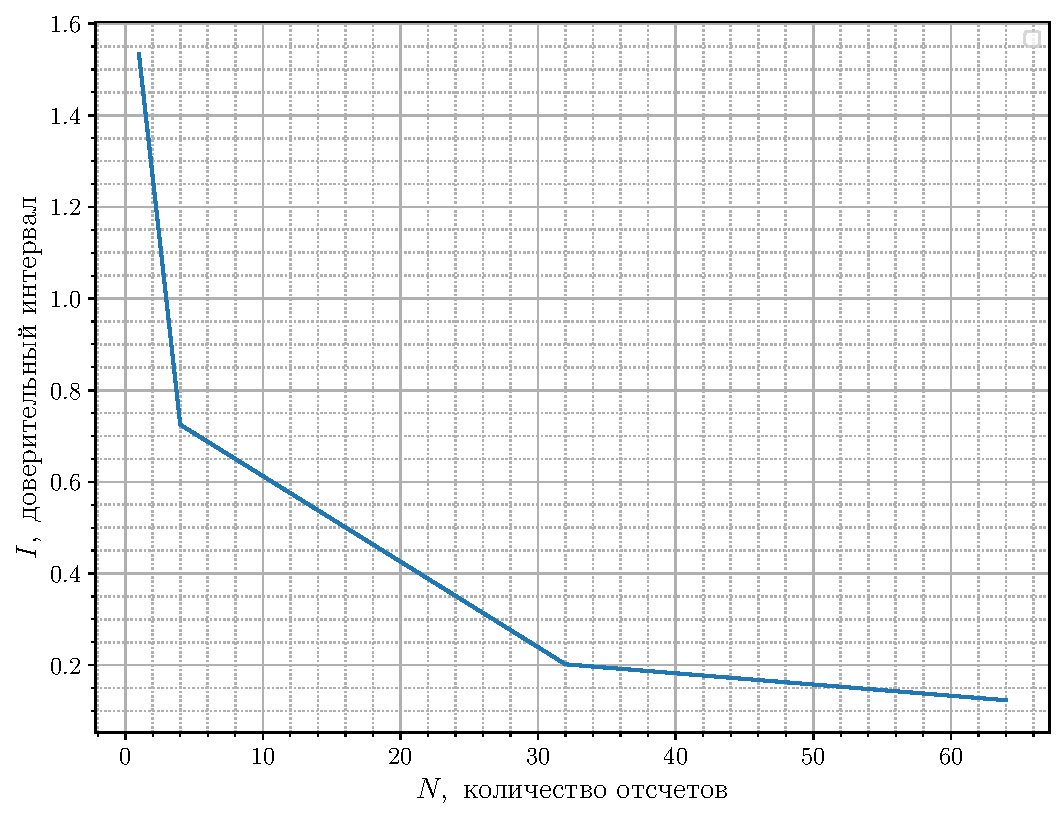
\includegraphics[width=0.8\linewidth]{fig/plot2}
	\caption*{График зависимости доверительного интервала $I$ от $N$}
	\end{figure}
\subsubsection[Задание 6.1]{Задание 6.2}
Доверительный интервал отмечается на графике тремя вертикальными линиями: центр интервала – зеленая линия, края интервала – левый край - красная линия, правый край – черная линия.
Порядок действий:
\begin{enumerate}
	\item Установили в Генераторе сигналов время корреляции Гауссова шума $\tau_\text{кор}=10$.
	\item В Усреднителе выбрали количество реализаций М = 256 (это необходимо для того, чтобы кривые зависимостей получались гладкими), доверительную вероятность $\beta = 0.95$, время между отсчетами $\Delta t = 1$ и необходимое количество отсчетов усреднения $N=1$. Доверительную вероятность выбирали последовательно равной $\beta = 0,80; 0,95; 0.98$.
	\item Нажали кнопку “PDF””. Значения доверительного интервала считывали в Блоке оценок. На основании полученных результатов представили зависимость $I_{\beta}(\beta)$.
	\item Получили аналогичные кривые для N=4, 32.
\end{enumerate}

 \begin{figure}[H]
	\begin{minipage}{0.3\linewidth}
		\centering
        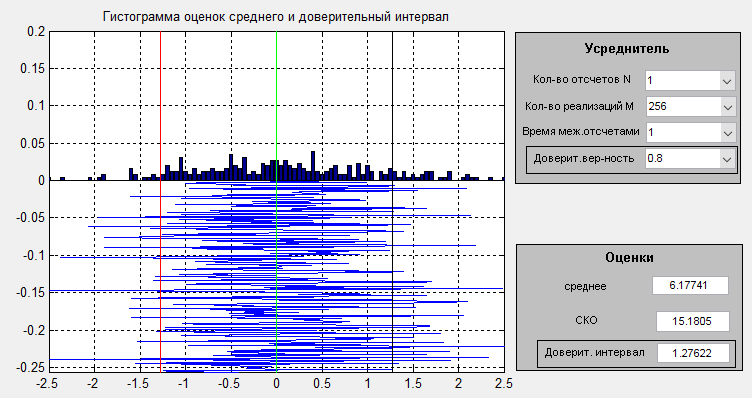
\includegraphics[width=\linewidth]{fig/realize_b1N1}
		\caption*{$\beta =0.8$}
	\end{minipage}
	\begin{minipage}{0.3\linewidth}
		\centering
        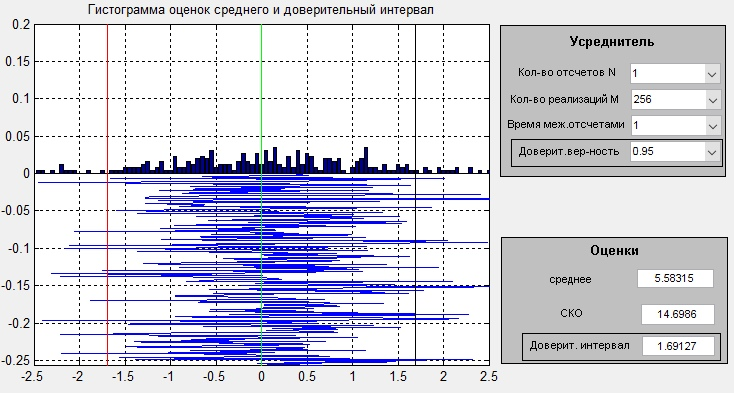
\includegraphics[width=\linewidth]{fig/realize_b2N1}
		\caption*{$\beta =0.95$}
	\end{minipage}
	\begin{minipage}{0.3\linewidth}
		\centering
        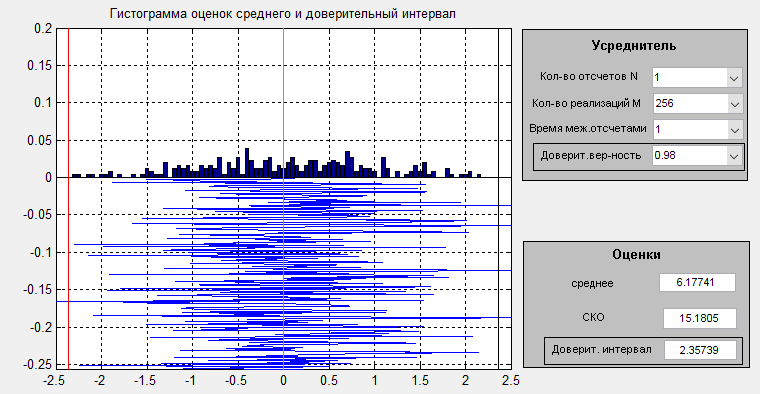
\includegraphics[width=\linewidth]{fig/realize_b3N1}
		\caption*{$\beta =0.98$}
	\end{minipage}
\caption*{$N=1$}
\end{figure}

 \begin{figure}[H]
	\begin{minipage}{0.3\linewidth}
		\centering
        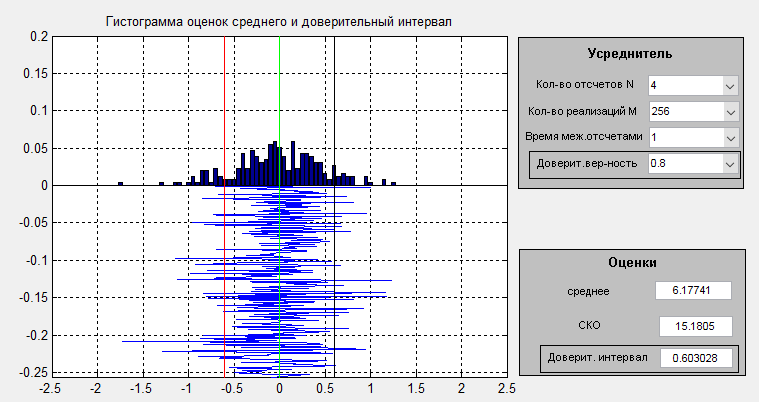
\includegraphics[width=\linewidth]{fig/realize_b1N2}
		\caption*{$\beta =0.8$}
	\end{minipage}
	\begin{minipage}{0.3\linewidth}
		\centering
        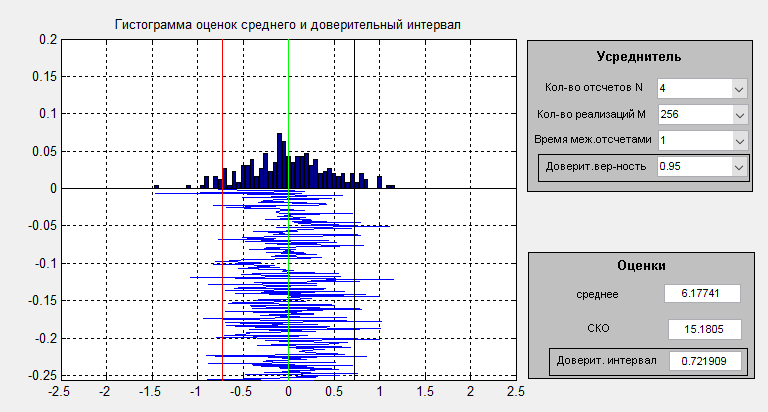
\includegraphics[width=\linewidth]{fig/realize_b2N2}
		\caption*{$\beta =0.95$}
	\end{minipage}
	\begin{minipage}{0.3\linewidth}
		\centering
        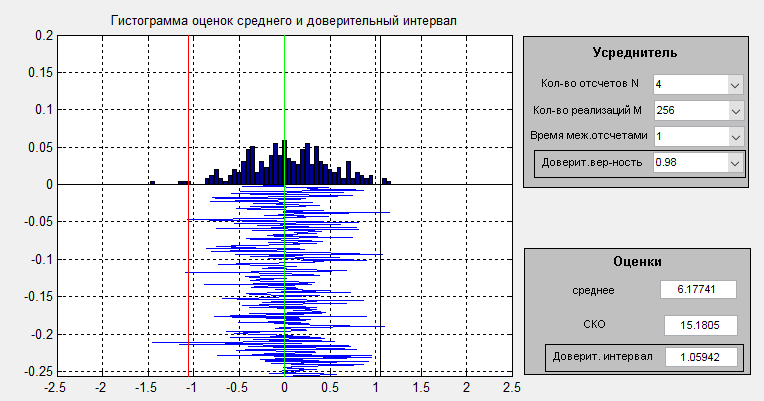
\includegraphics[width=\linewidth]{fig/realize_b3N2}
        \caption*{$\beta =0.98$}
	\end{minipage}
	\caption*{$N=4$}
	
\end{figure}
 \begin{figure}[H]
	\begin{minipage}{0.3\linewidth}
		\centering
        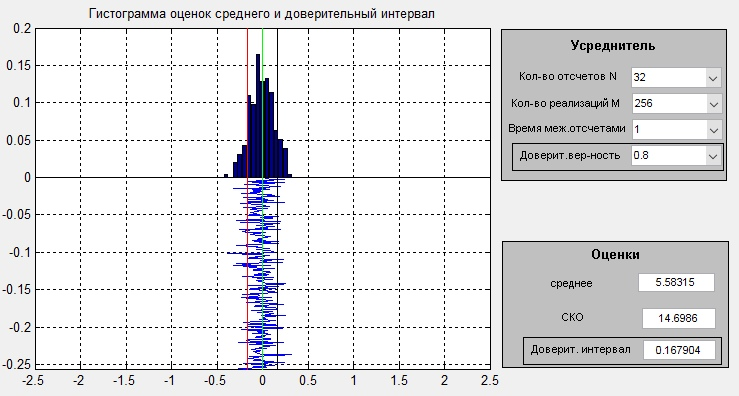
\includegraphics[width=\linewidth]{fig/realize_b1N3}
		\caption*{$\beta =0.8$}
	\end{minipage}
	\begin{minipage}{0.3\linewidth}
		\centering
        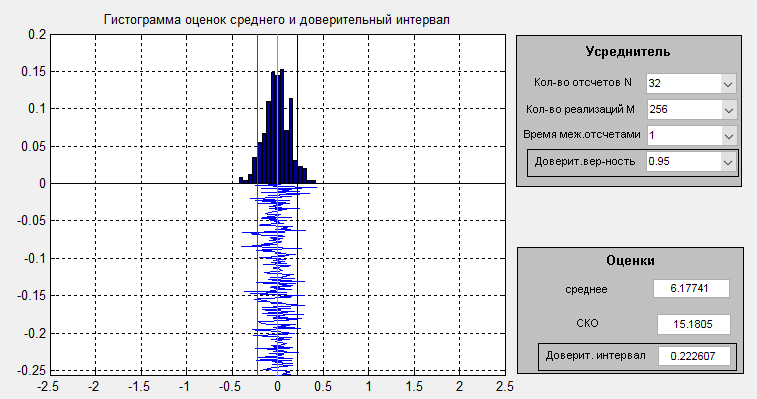
\includegraphics[width=\linewidth]{fig/realize_b2N3.png}
		\caption*{$\beta =0.95$}
	\end{minipage}
	\begin{minipage}{0.3\linewidth}
		\centering
        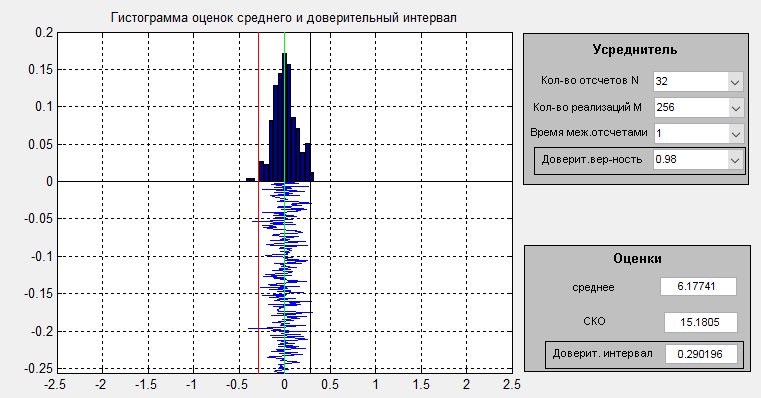
\includegraphics[width=\linewidth]{fig/realize_b3N3}
		\caption*{$\beta =0.98$}
	\end{minipage}
	\caption*{$N=32$}
\end{figure}
% Table generated by Excel2LaTeX from sheet 'Лист1'
\begin{table}[htbp]
	\centering
%	\caption{Add caption}
	\begin{tabular}{|c|c|c|c|}
		\toprule
		\multicolumn{1}{|c|}{} & \multicolumn{3}{c|}{Доверительный интервал I} \\
		\midrule
		\textbf{Доверительная вероятность $\beta$} & N=1 & N=4 & N=32 \\
		\midrule
		0.80  & 1.27622 & 0.603028 & 0.1809 \\
		\midrule
		0.95  & 1.69127 & 0.721909 & 0.2226 \\
		\midrule
		0.98  & 2.35739 & 1.05942  & 0.2901 \\
		\bottomrule
	\end{tabular}%
%	\label{tab:addlabel}%
\end{table}%
Построили график зависимости доверительного интервала $I$ от $\beta$ при различных значениях $N$.
 \begin{figure}[H]
	\centering
    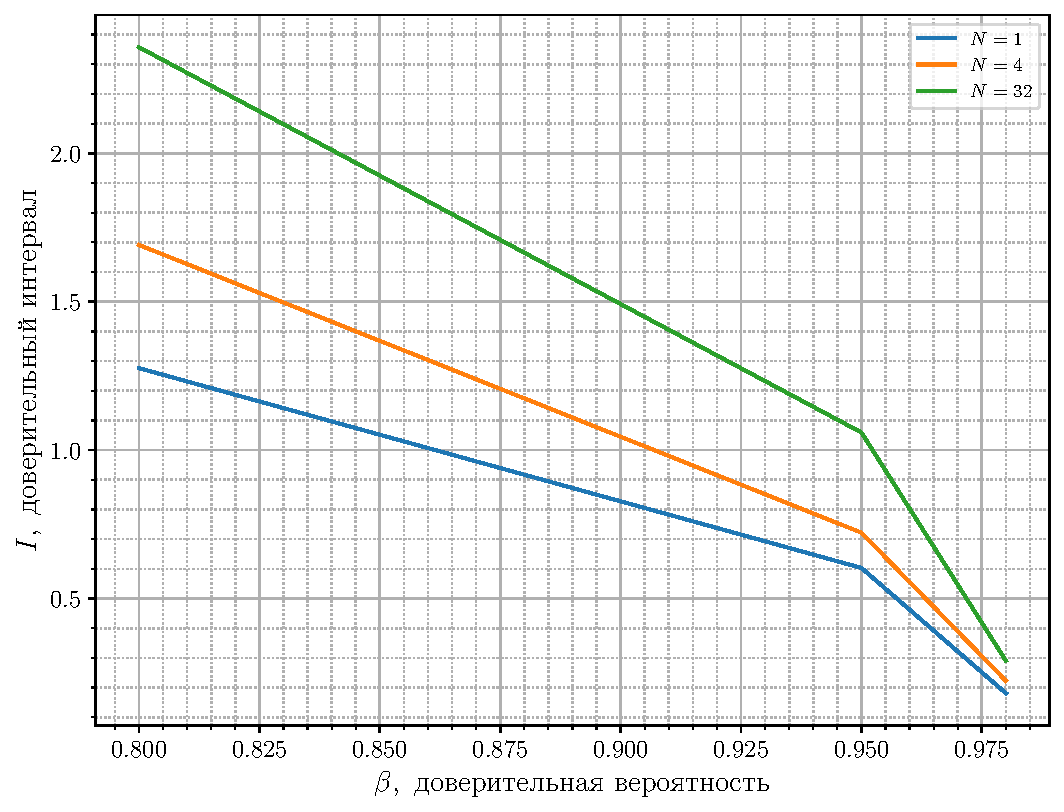
\includegraphics[width=0.8\linewidth]{fig/plot1}
	\caption*{График зависимости доверительного интервала $I$ от $\beta$}
\end{figure}
По графику видно, что доверительный интервал увеличивается при увеличении $\beta$ и уменьшается при увеличении количества отсчетов усреднения $N$.
\section{Вывод}
В результате выполнения данной работы мы изучили вопросы, связанные с оценкой параметров случайных процессов на примере оценки их средних значений
В ходе выполнения 1-го задания мы установили, что вид реализации с ростом времени корреляции становится более плавным, а спектральная плотность мощности смещается ближе к нулевой частоте.
Так же мы установили, что значения разброса $\mean{x}$ по вертикали во втором задании больше значений $\mean{x}$ из задания 5 при любых $N$.
В результате выполнения 6-го задания было установлено, что доверительный интервал увеличивается при увеличении $\beta$ и уменьшается при увеличении количества отсчетов усреднения $N$.

\end{document}
